\documentclass[a4paper,12pt]{article}  
\usepackage{geometry} 
\geometry{ 
 a4paper, 
 total={170mm,257mm}, 
 left=20mm, 
 top=20mm, 
} 
\usepackage{ wasysym }
\usepackage{titlesec} 
\titlelabel{\thetitle.\quad} %точка в section 
 
%%% Работа с русским языком 
\usepackage{cmap}                           % поиск в PDF 
\usepackage{mathtext}             % русские буквы в формулах 
\usepackage[T2A]{fontenc}               % кодировка 
\usepackage[utf8]{inputenc}              % кодировка исходного текста 
\usepackage[english,russian]{babel}  % локализация и переносы 
 
%Математика 
\usepackage{amsmath,amsfonts,amssymb,amsthm,mathtools} % AMS 
\usepackage{icomma} % "Умная" запятая 
 
%% Шрифты 
\usepackage{euscript}  % Шрифт Евклид 
\usepackage{mathrsfs} % Красивый матшрифт 
 
%% Команды 
\DeclareMathOperator{\const}{\mathop{const}} 
 
%% Перенос знаков в формулах 
%\newcommand*{\hm}[1]{#1\nobreak\discretionary{} 
% {\hbox{$\mathsurround=0pt #1$}}{}} 
\usepackage[pdftex]{graphicx} 
\usepackage{float} 
%%% Заголовок 
\author{Коротков Антон, Хохлов Андрей Б06-302} 
\title{Практическая работа 5 \\ 
 \textbf{Электрохимические процессы}} 
\date{\today} 
\begin{document} 
{\large\maketitle} 
\section{Сравнение химической активности металлов} 
В четыре пробирки налили по 1 мл 2М соляной кислоты и поместили в них 
металлические цинк, железо, медь и магний. Сравнили интенсивность выделения газа,результаты эксперимента занесли в табл 1 (в пробирку с железом добавили каплю 
красной кровяной соли для визуализации реакции) 
\begin{table}[h] 
\centering 
       \begin{tabular}{|l|l|l|l|l|} 
           \hline 
       Металл & \multicolumn{2}{|c|}{Mg} & \multicolumn{2}{|c|}{Zn}  \\ \hline 
        ~ & Наблюдения  & Реакция & Наблюдения  & Реакция  \\ \hline 
        HCl & Выделилось много газа & $\mathrm{H_2\uparrow}$ & Выделилось меньше газа &  $\mathrm{H_2\uparrow}$  \\ \hline 
    \end{tabular} 
\end{table} 
красной кровяной соли для визуализации реакции) 
\begin{table}[h] 
\centering 
       \begin{tabular}{|l|l|l|l|l|} 
    \hline 
       Металл & \multicolumn{2}{|c|}{Fe}& \multicolumn{2}{|c|}{Cu}   \\ \hline 
        ~ &Наблюдения  & Реакция & Наблюдения  & Реакция \\ \hline 
        HCl & Нет признаков реакции & Пассивирует & $\times$  & $\times$ \\ \hline 
    \end{tabular} 
\end{table} 
 
\begin{equation} 
\mathrm{Mg + HCl \longrightarrow MgCl_2 + H_2\uparrow } 
\end{equation} 
\begin{equation} 
\mathrm{Zn + HCl \longrightarrow ZnCl_2 + H_2\uparrow } 
\end{equation} 
\begin{equation} 
\mathrm{Fe + HCl \longrightarrow FeCl_2 + H_2\uparrow } 
\end{equation} 
\begin{equation} 
\mathrm{Cu + HCl \longrightarrow  } 
\end{equation} 
\begin{figure}[h] 
 
\centering 
 
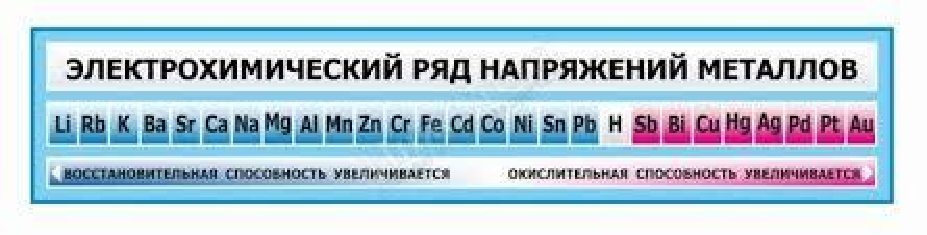
\includegraphics[scale=1]{series.pdf} 
 
\caption{Электрохимический ряд напряжений металлов} 
 
\label{fig:mpr} 
\end{figure}  
Экспериментальные данные сошлись с рядом электрохимического напряжения металлов.  
 
\section{Гальванический элемент} 
Механически очистили поверхность оцинкованного гвоздя и медной проволоки 
фильтровальной бумагой. В один химический стакан на 50 мл налили 1/2 объема 0,1М 
раствора сульфата цинка, а в другой – 0,1 М раствор сульфата меди. Соединили стаканы 
солевым мостиком (полоска фильтровальной бумаги), пропитанным раствором KCl (нас.), 
а электроды подсоединили к клеммам милливольтметра.выделение \textbf{газа}. 
 
\subparagraph{Составим схему гальванического элемента} 
 
\begin{equation} 
A(-) Zn^0 | ZnSO_4 || CuSO_4 | Cu^0 K(+)  
 \end{equation}
 
\subparagraph{Процессы на катоде:} $\mathrm{Cu^{2+}+2e^-=Cu^0}$
\subparagraph{Процессы на катоде:} $\mathrm{Zn^{0}-2e^-=Zn^{2+}}$
\begin{equation} 
ЭДС_{эксп}=\varepsilon_{эксп}=1.028В 
\end{equation} 
\begin{equation} 
\varepsilon_{теор}=\varepsilon_{B}-\varepsilon_{A}=0.34+0.76=1.1B 
\end{equation} 
 Элемент будет работать до тех пор, пока  ЭДС не уйдёт в ноль(пока разность электродных потенциалов не станет равна нулю  
\section{Определение электродного потенциала Cu2+/Cu} 
В химический стакан на 50 мл с небольшим количеством 1М раствора соли меди (II)
погрузили медный электрод и, предварительно закрепленный в штативе, хлорсеребряныйэлектрод
Измерили разность потенциалов между ними с помощью милливольтметра. Повторили опыт с растворами соли меди меньших концентраций: 0,1 М и 0,01 М. Записали
показания в табл. 5.2 и построили зависимость потенциала медного электрода отконцентрации электролита в полулогарифмических координатах, соответствующих
уравнению Нернста. Рассчитали стандартный потенциал медного электрода относительно стандартного хлорсеребряного электрода и пересчитали полученное
значение относительно стандартного водородного электрода. 
\begin{table}[!ht]
    \centering
    \begin{tabular}{|l|l|l|l|}
    \hline
        Концентрация раствора,М & $\log{C}$ & U, мВ & F, В \\ \hline
        0.01 & -2 & 0.103& 0.323 \\ \hline
        0.1 & -1 & 0.065 & 0.285\\ \hline
        1 & 0 & 0.052 & 0.272 \\ \hline
    \end{tabular}
\end{table}
\begin{equation}
    F_1=U_1+0.22=0.323 \newline
\end{equation}
\begin{equation}
     F_2=U_2+0.22=0.285
\end{equation}
\begin{equation}
     F_3=U_3+0.22=0.272\newline
\end{equation}
Табличные значения: $E_0(Ag/Cl)=0.22 E_0(Cu/Cu^{2+})=0.34В$
\begin{figure}[h] 
 
\centering 
 
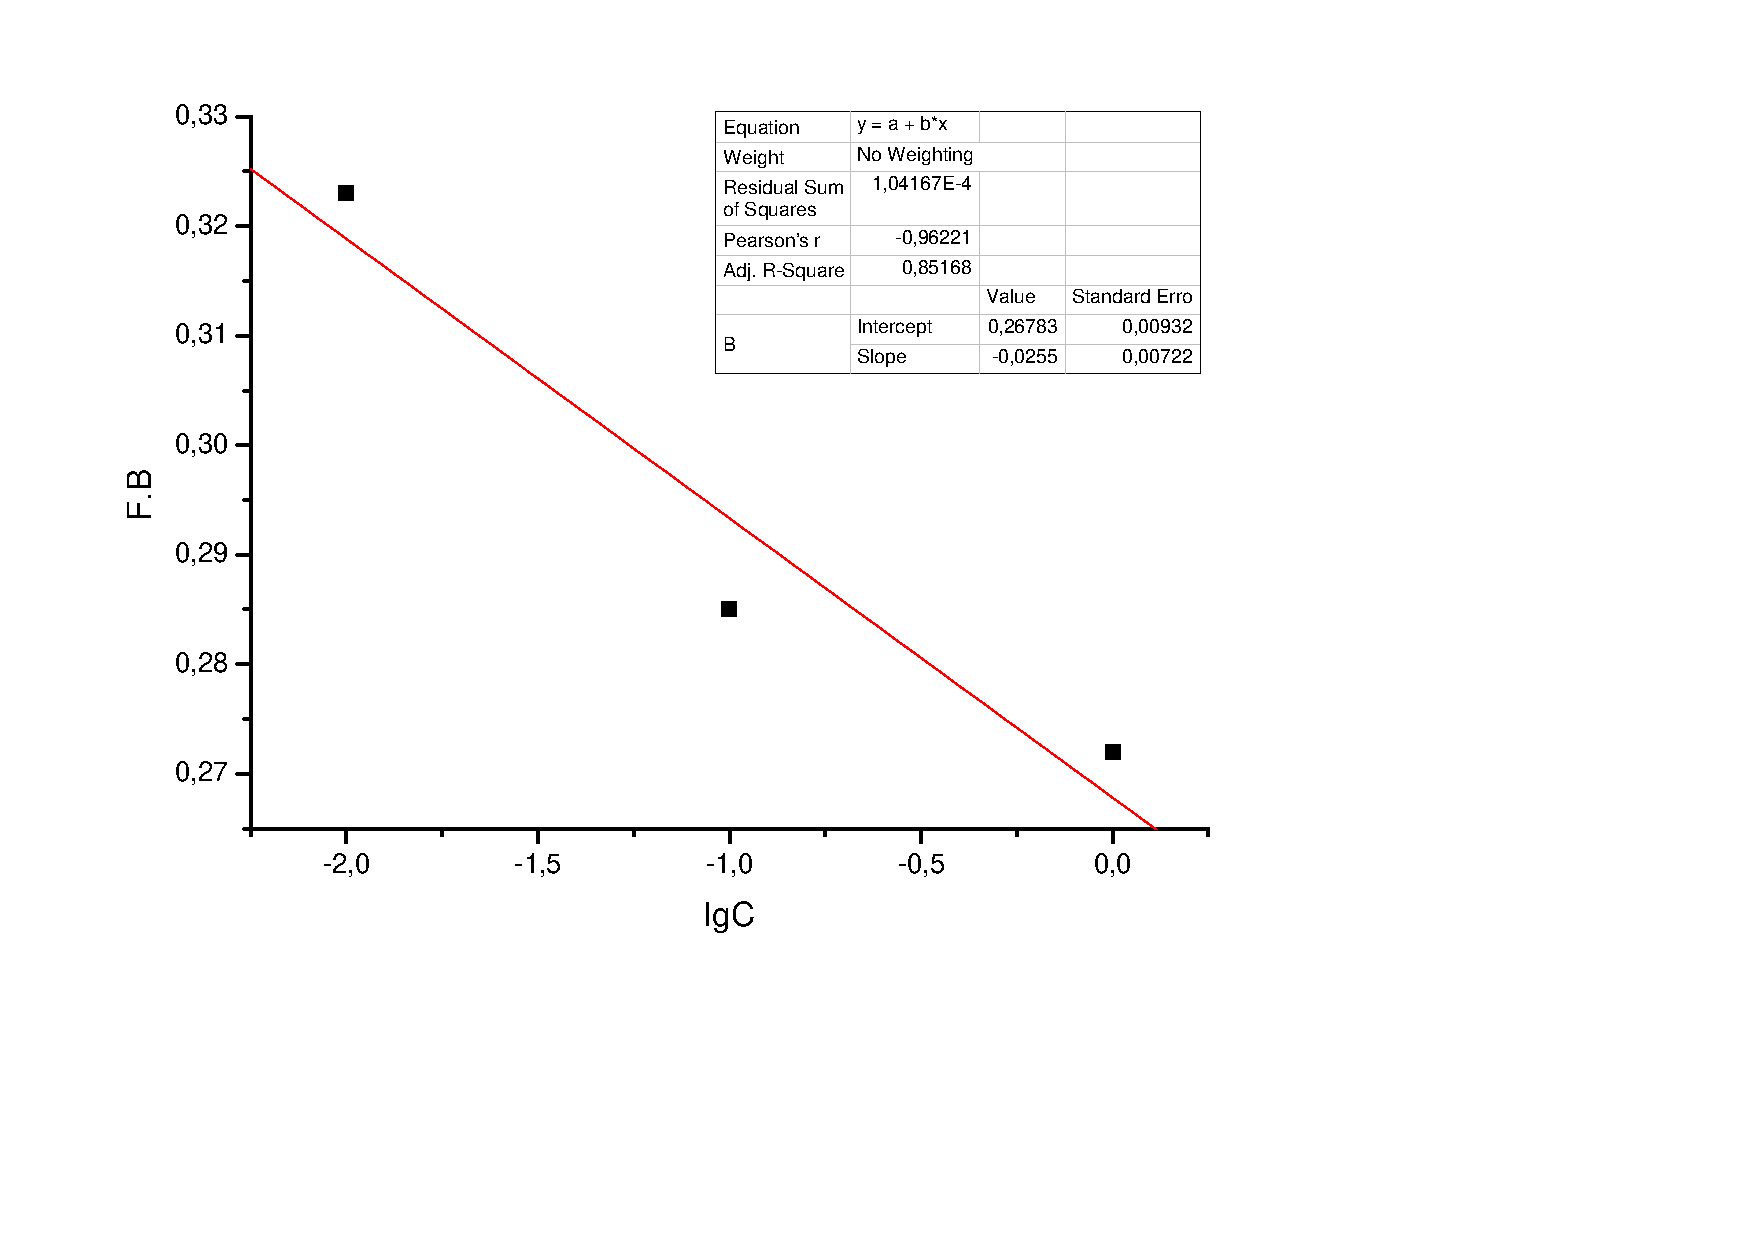
\includegraphics[scale=0.7]{nernst.pdf} 
 
\caption{Зависимость потенциала от логарифма} 
 
\label{fig:mpr} 
\end{figure}  
\section{Определение полярности источника питания с помощью электролизараствора поваренной соли}
В чашку Петри поместили фильтровальную бумажку, смоченную 0,1М раствором хлорида натрия и раствором фенолфталеина. Взяли источник постоянного тока
(батарея типа «Крона», 9 В) и коснулись оголенными контактами влажной части фильтровальной бумажки. На катоде (-) можно заметить проявление окраски фенолфталеина. 
\begin{equation}
    \mathrm{2NaCl+H_2O \longrightarrow 2NaOH+H_2\uparrow + Cl_2\uparrow}
\end{equation}
\subparagraph{Процессы на катоде:} $\mathrm{2H_2O+2e^-=H_2+OH^-}$
\subparagraph{Процессы на катоде:} $\mathrm{2Cl^--2e^-=Cl_2}$


Также можно использовать KI на йод-крахмальной бумаге для определения полярности, в процессе электролиза будет выделяться $I_2$,  и йод-крахмальная бумажка будет давать окраску.

\section{Электролиз растворов солей электролитов}
Заполнили стакан раствором 1М хлорида натрия и погрузили в него два инертных графитовых электрода
 В раствор добавили 3 капли фенолфталеина. Включили источник питания и установили ток электролиза 80–100 мА. 
 В процессе электролиза на катоде будет выделяться \textbf{водород} а на аноде \textbf{хлор}
 \begin{equation}
    \mathrm{2NaCl+H_2O \longrightarrow 2NaOH+H_2\uparrow + Cl_2\uparrow}
\end{equation}
\subparagraph{Процессы на катоде:} $\mathrm{2H_2O+2e^-=H_2+OH^-}$
\subparagraph{Процессы на катоде:} $\mathrm{2Cl^--2e^-=Cl_2}$

Если вместо поваренной соли использовать йодид калия, то на катоде будет выделяться  \textbf{водород}, а йод будет оставаться в растворе(ярко выраженный бурый цвет)
\begin{equation}
    \mathrm{2KI+H_2O \longrightarrow 2KOH+H_2\uparrow + I_2}
\end{equation}
\subparagraph{Процессы на катоде:} $\mathrm{2H_2O+2e^-=H_2+OH^-}$
\subparagraph{Процессы на катоде:} $\mathrm{2I^--2e^-=I_2}$


Йод будет реагировать с крахмалом и йод-крахмальная бумажка будет менять цвет.
\begin{figure}[h] 
 
\centering 
 
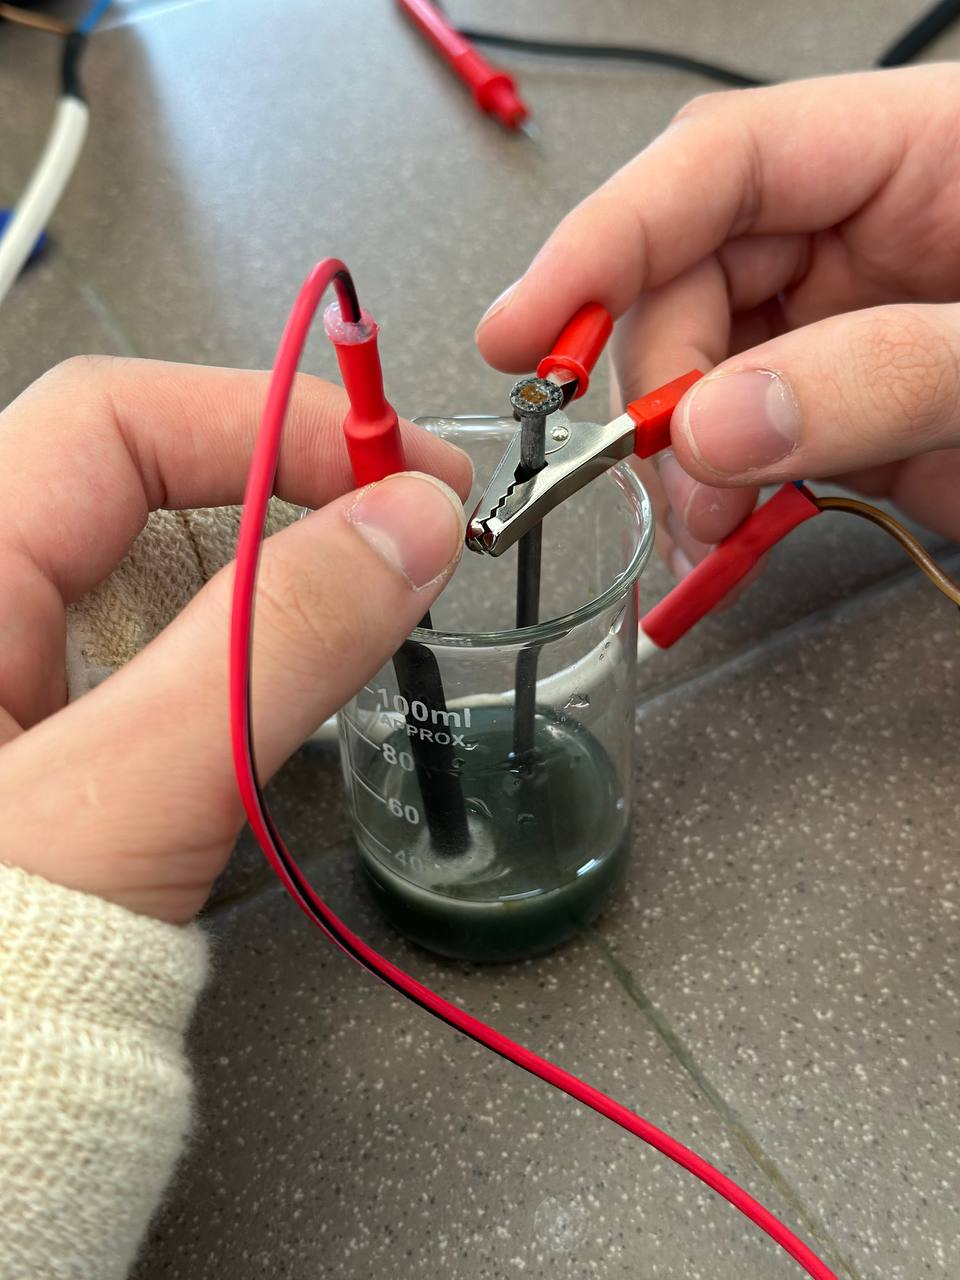
\includegraphics[scale=0.4]{elec.jpg} 
 
\caption{Установка для электролиза} 
 
\label{fig:mpr} 
\end{figure}  
\section{Получение водорода и кислорода электролизом. Закон Фарадея}
Собрали установку, изображенную на  В стакан на 100 мл (1) налили 60-
80 мл 1M NaOH. Поместили в стакан перевернутую пипетку (3) на 10-25 мл и погрузитестальные электроды (2) таким образом, чтобы один из электродов оказался внутри
пипетки. На верхний конец пипетки надели силиконовую трубку (4) с металлическим зажимом (5). С помощью спринцовки и зажима затянули раствор щелочи в пипетку до
одного из верхних делений (не до конца!). Убедились, что оба электрода (оголенныечасти) полностью погружены в раствор, а силиконовая трубка (клапан) закрыта
герметично (уровень жидкости не опускается).Подготовили источник постоянного тока на 5 В, амперметр, секундомер и
журнал для записи. Подключили электроды к источнику тока через амперметр(последовательно), выбрав полярность по указанию преподавателя. Отрегулировали
напряжение таким образом, чтобы протекающий ток составлял 80-120 мА. 
Делали электролиз в течение 10 мин , фиксируя значения тока в цепи каждые 30с.
После прекращения электролиза зафиксировали новый уровень жидкости
в пипетке. По разнице начального и конечного уровней определили объём выделившегося газа. (5 мл).
\begin{equation}
    \mathrm{H_2O \longrightarrow H_2\uparrow + O_2\uparrow}
\end{equation}
\subparagraph{Процессы на катоде:} $\mathrm{2H_2O+2e^-=H_2+OH^-}$
\subparagraph{Процессы на катоде:} $\mathrm{4OH^--4e^-=O_2+2H_2O}$
\begin{table}[H]    
\centering
    \begin{tabular}{|l|l|l|}
    \hline
    t(c) & I(mA) & m(мг) \\ \hline 
        60 & -98,1 & -0,48796 \\ \hline       
        120 & -98,6 & -0,98089 \\ \hline
        150 & -99 & -1,23109 \\ \hline       
        180 & -99,1 & -1,4788 \\ \hline
        210 & -99,33 & -1,72927 \\ \hline        
        240 & -99,4 & -1,9777 \\ \hline
        270 & -99,7 & -2,23163 \\ \hline        
        300 & -99,9 & -2,48456 \\ \hline
        330 & -100,2 & -2,74122 \\ \hline        
        360 & -100,4 & -2,99639 \\ \hline
        390 & -100,5 & -3,24933 \\ \hline        
        420 & -100,6 & -3,50276 \\ \hline
        450 & -100,8 & -3,76041 \\ \hline        
        480 & -101 & -4,01907 \\ \hline
        510 & -101,1 & -4,27449 \\ \hline        
        540 & -101,2 & -4,5304 \\ \hline
        570 & -101,3 & -4,78682 \\ \hline        
        600 & -101,5 & -5,0487 \\ \hline
    \end{tabular}
    \end{table}

    
    При эмпирическом рассчёте, масса выходит около \textbf{7мг}, погрешность измерения примерно \textbf{30 процентов}
    \section{Выводы}
    Жёстко заботали электрохимию.
\end{document}